Portfolio selection (or portfolio management) is the art and science of making decisions about investment mix and policy, matching investments to objectives, asset allocation for individuals and institutions, and balancing risk against performance. Modern Portfolio Theory (MPT) approaches investing by examining the entire market and the whole economy. The theory is an alternative to the older method of analyzing each investment’s individual merits. When investors look at each investment individual merit, they are analyzing an investment without worrying about the way different investments will perform in relation to each other. As a matter of fact, MPT places a large emphasis on the correlation between investments. Correlation is the amount we can expect various investments, and various asset classes, to change in value compared with each other. 

\section{Risk}
The term \textit{risk} is defined as the measurement of the likelihood that an investment will go up and down in value, how often and by how much. The theory assumes that investors prefer to minimize risk; in fact, it assumes that given the choice of two portfolios with equal returns, investors will choose the one with the least risk. If investors take on additional risk, they will expect to be compensated with additional return. Risk comes in two major categories:
\begin{itemize}
\item \textbf{Systematic risk} - the possibility that the entire market and economy will show losses, which will negatively affect nearly every investment; also called \textit{market risk};
\item \textbf{Unsystematic risk} – the possibility that an investment or a category of investments will decline in value without having a major impact upon the entire market
\end{itemize}
Diversification generally does not protect against systematic risk because a drop in the entire market and economy typically affects all investments. However, diversification is designed to decrease unsystematic risk. Since unsystematic risk is the possibility that one single thing will decline in value, having a portfolio invested in a variety of stocks, a variety of asset classes and a variety of sectors will lower the risk of losing much money when one investment type declines in value. Figure (\ref{fig:div}) shows how diversification strategies can reduce the overall risk of the invested portfolio.

\begin{figure}
\centering
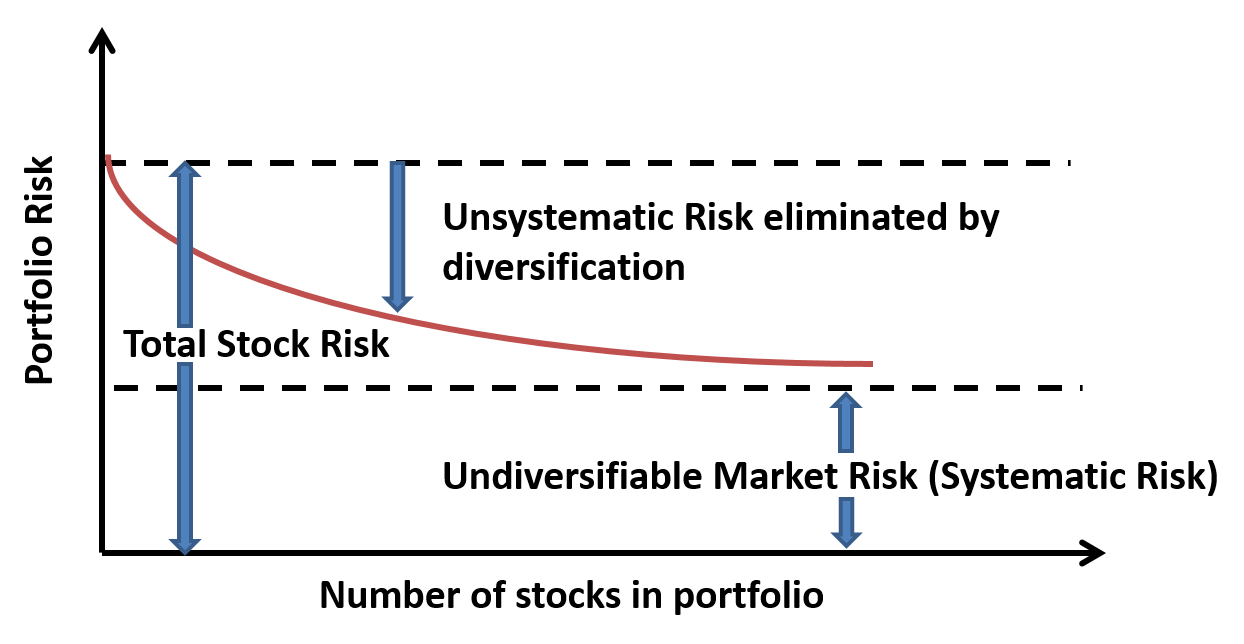
\includegraphics[scale=0.6]{Diversification} 
\caption{How the diversification can reduce the overall risk}
\label{fig:div}
\end{figure}

\section{Markovitz Theory}
Consider a portfolio with $n$ different assets where asset number $i$ will give the return $R_i$. Let $\mu_i$ and $\sigma^2_i$ be the corresponding mean and variance and assume, for any two assets $i$ and $j$ that is known their correlation coefficient $\rho_{ij}$. Let $\sigma_{i,j} = \rho_{ij}\sigma_i\sigma_j$ be the covariance between $R_i$ and $R_j$. Suppose the the relative amount of the value of the portfolio invested in asset $i$ is $x_i$. If $R$ is the return of the whole portfolio then:
\begin{equation}
\mu = E[R] = \sum\limits_{i=1}^n\mu_i x_i 
\end{equation}
\begin{equation}
\sigma^2 = Var[R] = \sum\limits_{i=1}^n\sum\limits_{j=1}^n\sigma_{i,j}x_i x_j = x^T \Sigma x
\end{equation}
where $\Sigma$ is the covariance matrix and $\Sigma_{ij} = \sigma_{i,j}x_i x_j$ \cite{markovitz}.
For different choices of $x_1, ..., x_n$ the investor will get different combinations of $\mu$ and $\sigma^2$. The set of all possible ($\sigma^2$, $\mu$) combinations is called the \textit{attainable set}. Those ($\sigma^2$, $\mu$) with minimum $\sigma^2$ for a given $\mu$ or more and maximum $\mu$ for a given $\sigma^2$ or less are called the \textit{efficient set} (or efficient frontier). Since an investor wants a high profit and a small risk, he wants to maximize $\mu$ and minimize $\sigma^2$ and should therefore choose a portfolio which gives a ($\sigma^2$, $\mu$) combination in the efficient set. In Figure (\ref{fig:efficient}) the attainable set is the interior of the ellipse and the efficient set is the upper left part of its boundary. \\
\begin{figure}
\centering
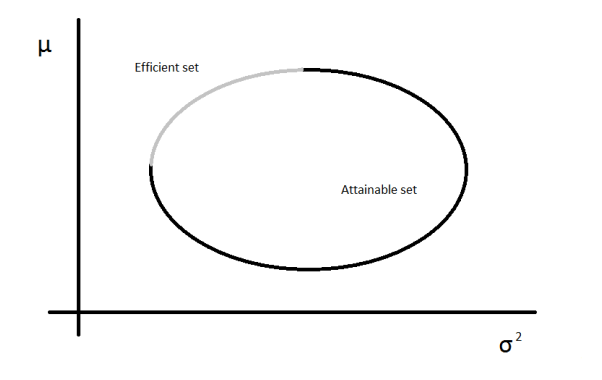
\includegraphics[scale=0.9]{efficient_set} 
\caption{The efficient set in the ($\sigma^2$,$\mu$) plane}
\label{fig:efficient}
\end{figure}

\section{Sharpe Ratio (SR)}
The Sharpe Ratio is a measure for calculating risk-adjusted return \cite{sharpe}. The Sharpe Ratio is the average return earned in excess of the \textit{risk-free rate} per unit of volatility or total risk. Subtracting the \textit{risk-free rate} from the mean return, the performance associated with risk-taking activities can be isolated:
\begin{equation}\label{eq:SR}
SR(x) = \frac{\mu(x) - \mu_{RF}}{\sigma(x)}
\end{equation} 
where $\mu(x)$ is the expected return of the invested portfolio, $\mu_{RF}$ is the \textit{risk-free rate} and $\sigma(x)$ is the portfolio standard deviation ($\sqrt{x^T \Sigma x}$). The greater a portfolio's Sharpe Ratio, the better its risk-adjusted performance has been. A negative Sharpe Ratio indicates that a risk-less asset would perform better than the security being analyzed.

\section{Diversification Ratio (DR)}
The \textit{Diversification Ratio} (DR) is a measure of a portfolio diversification, defined as the ratio of the portfolio’s weighted
average volatility to its overall volatility \cite{diversification}. Formally, if $x$ is the vector of the assets' weights,
\begin{equation}\label{eq:dr}
DR(x) = \frac{\sum_{i=1}^{n}x_i\sigma_i}{\sigma(x)}
\end{equation}
It is intuitive that portfolios with “concentrated” weights and/or highly correlated holdings would be poorly diversified, and hence be characterized by relatively low DRs.

\section{Portfolio selection}
The Markowitz portfolio theory states that an investor should
choose a portfolio from the efficient set, depending on how risk averse he is. One way to handle this, is to consider the optimization problem\footnotemark[1]\footnotetext[1]{The condition $x \geq 0$ is often referred as \textit{long-only} investment strategy.}:
\begin{equation}
\begin{aligned}
&\min_x &&(\sigma^2 - A\mu) = x^T \Sigma x - A\mu^T x\\
&\text{s.t.}&&\mathds{1}^T x=1\\
&&&x \geq 0
\end{aligned}
\end{equation}

where $\mathds{1} = [1, .., 1] \in \mathbb{R}^n$ is the vector of all ones and $A$ ($0 \leq A \leq \infty$) is the so called \textit{risk aversion index}. $A = 0$ will result in the portfolio with the \textit{smallest variance}. An increasing $A$ corresponds to the investor becoming more willing to take a bigger risk to get a higher expected return; $A = \infty$ corresponds to the investor only caring about getting a large expected return no matter what the risk is \cite{markovitz}.\\
If we set $A=0$, the problem became a \textit{mean-variance
optimization} (MVO) problem. If we add the constraint that every asset yields at least a target value $R$ of expected return, we obtain a convex quadratic programming problem:
\begin{equation}\label{eq:variance}
\begin{aligned}
&\min_x &&\frac{1}{2}x^T \Sigma x\\
&\text{s.t.}
&&\mu^T x \geq R\\
&&&\mathds{1}^T x=1\\
&&&x \geq 0
\end{aligned}
\end{equation}
Note that the matrix $\Sigma$ is positive semidefinite since $x^T \Sigma x$, the variance of the portfolio, must be nonnegative for every portfolio (feasible or not) $x$.\\
An alternative way to formulate the MVO problem is the following:
\begin{equation}\label{eq:variance2}
\begin{aligned}
&\max_x &&\mu^Tx\\
&\text{s.t.}
&&x^T \Sigma x \leq \sigma^2\\
&&&\mathds{1}^T x=1\\
&&&x \geq 0
\end{aligned}
\end{equation}

While in (\ref{eq:variance}) we attempt to minimize the variance of the portfolio, with the constraint that the return is at least greater than a fixed value of return $R$, in (\ref{eq:variance2}) we try to maximize the return, constraining the variance to be less or equal than a certain fixed value $\sigma^2$ \cite{libro}.\\
The main problems of the mean-variance approach are two. The first is that there is no reason to expect that solutions to the Markowitz model will be well diversified portfolios. Diversification means reducing \textit{risk} by investing in a variety of assets. This model tends to produce portfolios with unreasonably large weights in certain asset classes \cite{libro}. The second criticism of the Markovitz model is its sensitivity to inputs \cite{tutuncu}.